%% =====================================================================
%%  TEMPLATE DE SUBMISSAO -- XVIII COMPUTER ON THE BEACH (COTB 2027)
%%  Florianopolis - SC, 13 a 17 de abril de 2027
%% =====================================================================
%%
%%  VERSAO CORRIGIDA PARA USO NO OVERLEAF (IFSC Garopaba, PI-II, 10/2026)
%%  ----------------------------------------------------------------
%%  Este arquivo reproduz o template oficial publicado em
%%  https://computeronthebeach.com.br/trilha-principal.html
%%  (arquivo template_cotb2027.tex), com tres correcoes:
%%    - os acentos do arquivo original estavam gravados como entidades
%%      HTML (ex.: "Introdu&ccedil;&atilde;o"), o que impede a
%%      compilacao; aqui estao como caracteres UTF-8 normais;
%%    - a imagem "figura_exemplo.png", usada no exemplo de figura,
%%      nao era distribuida; agora acompanha o projeto;
%%    - o comentario das referencias citava 8 paginas para Artigo
%%      Completo; o limite oficial e de 6 paginas.
%%  A classe, as margens e a formatacao nao foram alteradas.
%%  Na duvida, vale o que estiver publicado no site do evento.
%%
%%  INSTRUCOES GERAIS DE USO DESTE TEMPLATE
%%  ----------------------------------------------------------------
%%  1. TRILHAS DE SUBMISSAO
%%     (a) ARTIGO COMPLETO: deve descrever atividades de pesquisa,
%%         relatos de experiencias relevantes e estudos de caso.
%%         Limite: MAXIMO DE 6 (SEIS) PAGINAS, incluindo todas as
%%         secoes do template (introducao, desenvolvimento, resultados,
%%         conclusao E REFERENCIAS). Os artigos aceitos serao
%%         apresentados oralmente em sessoes tecnicas.
%%     (b) RESUMO ESTENDIDO: deve descrever trabalhos em andamento,
%%         ainda sem resultados consolidados. Limite: MAXIMO DE 3
%%         (TRES) PAGINAS, incluindo todas as secoes do template
%%         (incluindo referencias). Os trabalhos aceitos serao
%%         apresentados em sessoes de posteres.
%%
%%     ATENCAO: cada trabalho pode ser submetido a APENAS UMA trilha.
%%     Um mesmo trabalho nao pode ser enviado simultaneamente para
%%     Artigos Completos, Resumos Estendidos e/ou para o Concurso de
%%     Trabalhos Tecnicos. A submissao duplicada em mais de uma
%%     trilha acarreta a DESCLASSIFICACAO do trabalho.
%%
%%  2. IDIOMA
%%     O corpo do artigo (texto principal) pode ser escrito em
%%     Portugues, Espanhol ou Ingles.
%%
%%     OBRIGATORIO PARA TODOS OS TRABALHOS, independentemente do
%%     idioma do texto principal:
%%       - TITULO EM INGLES;
%%       - ABSTRACT EM INGLES;
%%       - KEYWORDS EM INGLES.
%%     Alem disso, se o trabalho for escrito em Portugues ou em
%%     Espanhol, o TITULO TAMBEM DEVE APARECER NO IDIOMA DO ARTIGO
%%     (ou seja, o trabalho tera DOIS TITULOS: um em ingles e outro
%%     no idioma em que o artigo foi escrito). Se o artigo for
%%     escrito em ingles, um unico titulo (em ingles) e suficiente.
%%     Veja a secao "TITULO" mais abaixo neste arquivo para o uso
%%     pratico dos comandos \title e \translatedtitle.
%%
%%  3. FORMATO DE SUBMISSAO
%%     A submissao deve ser feita EXCLUSIVAMENTE em formato PDF,
%%     gerado a partir deste template LaTeX (ou do template .docx
%%     equivalente, quando disponibilizado pela organizacao).
%%
%%  4. DUAS VERSOES OBRIGATORIAS DO ARQUIVO
%%     (a) VERSAO PARA AVALIACAO (ANONIMA / "BLIND REVIEW"):
%%         - NAO deve conter nomes dos autores, afiliacoes, e-mails
%%           ou quaisquer outros dados que permitam identifica-los.
%%         - A secao de AGRADECIMENTOS deve ser removida ou mantida
%%           de forma anonimizada (ex.: "Agradecimentos omitidos
%%           para avaliacao cega.").
%%         - Evite tambem autocitacoes que revelem a autoria
%%           (ex.: "em nosso trabalho anterior [12]..."); prefira
%%           formas neutras de citacao.
%%         - Para gerar esta versao, use a opcao "anonymous" da
%%           classe acmart (ver linha de \documentclass abaixo).
%%     (b) VERSAO FINAL (CAMERA-READY):
%%         - Deve conter a identificacao COMPLETA de todos os
%%           autores (nome, afiliacao, endereco, cidade, pais e
%%           e-mail institucional).
%%         - Deve incluir a secao de AGRADECIMENTOS completa.
%%         - Deve incluir a DECLARACAO DE USO DE INTELIGENCIA
%%           ARTIFICIAL GENERATIVA (obrigatoria em ambas as
%%           versoes -- ver secao correspondente ao final deste
%%           template).
%%
%%  5. ESTRUTURA MINIMA OBRIGATORIA (todas as secoes contam para o
%%     limite de paginas da trilha escolhida):
%%       - Titulo, resumo (abstract) e palavras-chave
%%       - Introducao
%%       - Fundamentacao Teorica / Trabalhos Relacionados
%%       - Materiais e Metodos (ou Desenvolvimento)
%%       - Resultados (quando aplicavel -- opcional apenas para
%%         Resumo Estendido, que pode apresentar resultados
%%         preliminares ou esperados)
%%       - Discussao
%%       - Conclusao e Trabalhos Futuros
%%       - Agradecimentos (anonimizados na versao de avaliacao)
%%       - Declaracao de Uso de Inteligencia Artificial
%%       - Referencias
%%
%%  6. CLASSE LATEX UTILIZADA (acmart)
%%     ---------------------------------------------------------------
%%     Este template usa a classe "acmart" (formato ACM sigconf, em
%%     duas colunas). O Overleaf ja traz a classe acmart e o estilo
%%     ACM-Reference-Format instalados: nao e preciso enviar nenhum
%%     arquivo .cls ou .bst para o projeto.
%%
%%  7. COMO USAR ESTE ARQUIVO
%%     - Substitua todos os campos entre colchetes [ ] pelo conteudo
%%       do seu trabalho.
%%     - Nao altere a classe de documento, margens, fontes ou
%%       comandos de formatacao do template.
%%     - Os exemplos de figura, tabela, formula e citacao presentes
%%       neste arquivo servem apenas como referencia de formatacao;
%%       remova-os e substitua pelo conteudo real do seu trabalho.
%%     - Remova os comentarios de instrucao (linhas iniciadas por %%)
%%       antes da submissao final, mantendo apenas o conteudo do
%%       artigo.
%% =====================================================================


%% ---------------------------------------------------------------
%% ESCOLHA DA VERSAO:
%%  - Para a VERSAO DE AVALIACAO (anonima), use a linha com a opcao
%%    "anonymous" (descomente-a e comente a outra).
%%  - Para a VERSAO FINAL (camera-ready), use a linha sem "anonymous".
%%
%% As opcoes "language=..." abaixo habilitam o recurso nativo da
%% classe acmart para TITULO EM DOIS IDIOMAS (comando
%% \translatedtitle, usado mais abaixo). "language={main=english}"
%% garante que o INGLES continue sendo o idioma padrao do documento
%% (usado nos rotulos automaticos "Abstract"/"Keywords", cabecalhos
%% etc.), mesmo com portugues e espanhol tambem habilitados para uso
%% no corpo do texto e no titulo traduzido.
%% ---------------------------------------------------------------
%\documentclass[sigconf, nonacm, screen, anonymous, language=portuguese, language=spanish, language={main=english}]{acmart} % VERSAO DE AVALIACAO
\documentclass[sigconf, nonacm, screen, language=portuguese, language=spanish, language={main=english}]{acmart}             % VERSAO FINAL

\AtBeginDocument{%
  \providecommand\BibTeX{{%
    \normalfont B\kern-0.5em{\scshape i\kern-0.25em b}\kern-0.8em\TeX}}}

%% NAO carregue o pacote babel manualmente: a classe acmart ja o
%% carrega automaticamente com os idiomas indicados nas opcoes
%% "language=..." do \documentclass acima (evita conflito de dupla
%% carga do babel).
\usepackage{amsmath}
\usepackage{amsfonts}
\let\Bbbk\relax
\usepackage{amssymb}
\usepackage{booktabs}
\usepackage{multirow}
\usepackage{graphicx}

%% Remove o bloco de identificacao ACM (nao se aplica ao evento)
\settopmatter{printccs=false, printacmref=false}
\renewcommand\footnotetextcopyrightpermission[1]{}

%% =====================================================================
%% CABECALHO PERSONALIZADO (dados do evento a esquerda, autores a
%% direita)
%% ---------------------------------------------------------------------
%% - O lado ESQUERDO do cabecalho traz o nome/edicao do evento, local
%%   e datas. Edite a macro \cotbEventInfo abaixo se necessario.
%% - O lado DIREITO do cabecalho traz os autores do trabalho:
%%     * ate 3 (tres) autores: lista todos os nomes (gerado
%%       automaticamente a partir dos comandos \author usados mais
%%       abaixo, no mesmo formato usado pela classe acmart);
%%     * mais de 3 (tres) autores: exibe apenas o PRIMEIRO autor
%%       seguido de "et al." (tambem gerado automaticamente).
%%   Nao e necessario editar nada manualmente: o comportamento eh
%%   determinado pela quantidade de comandos \author preenchidos
%%   na secao de autores, logo abaixo.
%% =====================================================================
\makeatletter
\newcounter{cotbNumAuthors}
\let\cotb@originalauthor\author
\renewcommand{\author}[1]{%
  \stepcounter{cotbNumAuthors}%
  \ifnum\value{cotbNumAuthors}=1
    \gdef\cotbFirstAuthorName{#1}%
  \fi
  \cotb@originalauthor{#1}%
}
\makeatother

%% Dados do evento exibidos do lado esquerdo do cabecalho (mantenha
%% o texto curto, em ate duas linhas, para nao colidir com o lado
%% direito):
\newcommand{\cotbEventInfo}{XVIII Computer on the Beach (COTB 2027)\\
  Florianópolis/SC --- 13 a 17 de abril de 2027}

%% Autores exibidos do lado direito do cabecalho (logica automatica
%% de "et al." para mais de 3 autores):
\newcommand{\cotbHeaderAuthors}{%
  \ifnum\value{cotbNumAuthors}>3
    \cotbFirstAuthorName\ et al.%
  \else
    \shortauthors
  \fi
}

%% Espaco reservado para o cabecalho de duas linhas nao colidir com
%% o corpo do texto:
\setlength{\headheight}{24pt}

\AtBeginDocument{%
  \fancypagestyle{firstpagestyle}{%
    \fancyhf{}%
    \renewcommand{\headrulewidth}{0.4pt}%
    \renewcommand{\footrulewidth}{0pt}%
    \fancyhead[L]{\begin{minipage}[b]{0.62\textwidth}\raggedright
      \scriptsize\cotbEventInfo\end{minipage}}%
    \fancyhead[R]{\begin{minipage}[b]{0.34\textwidth}\raggedleft
      \scriptsize\cotbHeaderAuthors\end{minipage}}%
    \fancyfoot[C]{\if@ACM@printfolios\thepage\fi}%
  }%
  \fancypagestyle{standardpagestyle}{%
    \fancyhf{}%
    \renewcommand{\headrulewidth}{0.4pt}%
    \renewcommand{\footrulewidth}{0pt}%
    \fancyhead[L]{\begin{minipage}[b]{0.62\textwidth}\raggedright
      \scriptsize\cotbEventInfo\end{minipage}}%
    \fancyhead[R]{\begin{minipage}[b]{0.34\textwidth}\raggedleft
      \scriptsize\cotbHeaderAuthors\end{minipage}}%
    \fancyfoot[C]{\if@ACM@printfolios\thepage\fi}%
  }%
  %% IMPORTANTE: a classe acmart ja executa "\pagestyle{standardpagestyle}"
  %% durante o carregamento (antes desta redefinicao ter efeito). Por
  %% isso, e necessario chamar \pagestyle novamente aqui, para que o
  %% cabecalho das paginas internas passe a usar a versao customizada
  %% definida acima (evento a esquerda, autores a direita).
  \pagestyle{standardpagestyle}%
}

\begin{document}

%% =====================================================================
%% TITULO
%% ---------------------------------------------------------------------
%% \title{...}  -> OBRIGATORIO EM INGLES para todos os trabalhos,
%%                 independentemente do idioma do artigo.
%% \translatedtitle{idioma}{...} -> use APENAS se o artigo for escrito
%%                 em Portugues ou Espanhol, informando o titulo
%%                 tambem no idioma do artigo (o trabalho passa a ter
%%                 DOIS TITULOS, exibidos um abaixo do outro, com a
%%                 mesma formatacao). Use "portuguese" ou "spanish"
%%                 como idioma, conforme o caso. Se o artigo for
%%                 escrito em Ingles, NAO utilize \translatedtitle
%%                 (um unico titulo, em ingles, e suficiente).
%% =====================================================================
\title{[Title of the Paper in English]}
\translatedtitle{portuguese}{[Título do Trabalho em Português]}
%% Caso o artigo seja em Espanhol, troque a linha acima por:
%% \translatedtitle{spanish}{[Título del Trabajo en Español]}
%% Caso o artigo seja em Ingles, apague ou comente a linha \translatedtitle.

%% =====================================================================
%% AUTORES
%% ---------------------------------------------------------------------
%% NA VERSAO DE AVALIACAO (anonima): remova ou comente TODOS os blocos
%% de \author, \affiliation e \email abaixo. Com a opcao "anonymous"
%% da classe acmart ja habilitada, a compilacao substitui os dados
%% por identificadores neutros, mas recomenda-se tambem nao deixar
%% nenhuma informacao de identificacao no codigo-fonte.
%%
%% NA VERSAO FINAL: preencha os dados completos de todos os autores,
%% um bloco \author/\affiliation/\email para cada um.
%% =====================================================================
\author{[Nome Completo do Primeiro Autor]}
\affiliation{%
  \institution{[Instituicao do Autor]}
  \streetaddress{[Endereco]}
  \city{[Cidade]}
  \state{[Estado]}
  \country{[Pais]}}
\email{[email@instituicao.br]}

\author{[Nome Completo do Segundo Autor]}
\affiliation{%
  \institution{[Instituicao do Autor]}
  \streetaddress{[Endereco]}
  \city{[Cidade]}
  \state{[Estado]}
  \country{[Pais]}}
\email{[email@instituicao.br]}

%% Adicione quantos blocos de \author forem necessarios.


%% =====================================================================
%% RESUMO / ABSTRACT
%% ---------------------------------------------------------------------
%% OBRIGATORIO EM INGLES para todos os trabalhos, independentemente
%% do idioma do artigo (Portugues, Espanhol ou Ingles). Escreva um
%% resumo de ate ~250 palavras, indicando problema, objetivo,
%% metodo, principais resultados e contribuicao. Para Resumo
%% Estendido, indique que o trabalho esta em andamento e destaque
%% resultados esperados ou preliminares.
%% =====================================================================
\begin{abstract}
[Write here a concise abstract (up to approximately 250 words)
describing the problem addressed, the objective of the work, the
methodology employed, the main results obtained, and the
contribution of the study. For an Extended Abstract, indicate that
the work is in progress and highlight expected or preliminary
results.]
\end{abstract}

%% =====================================================================
%% PALAVRAS-CHAVE / KEYWORDS
%% OBRIGATORIO EM INGLES para todos os trabalhos, independentemente
%% do idioma do artigo.
%% =====================================================================
\keywords{[Keyword 1], [Keyword 2], [Keyword 3], [Keyword 4]}

\maketitle

%% Selecione abaixo o idioma principal do CORPO DO TEXTO (o restante
%% do artigo, a partir daqui). Use "portuguese", "spanish" ou
%% "english", conforme o idioma escolhido para o artigo. Isso NAO
%% afeta o titulo/abstract/keywords acima, que seguem sempre as
%% regras da secao "IDIOMA" no topo deste arquivo.
\selectlanguage{portuguese}

%% =====================================================================
%% 1. INTRODUCAO
%% Contextualize o tema, apresente o problema de pesquisa, a
%% motivacao, os objetivos do trabalho e a organizacao do artigo.
%% =====================================================================
\section{Introdução}
[Texto da introdução...]


%% =====================================================================
%% 2. FUNDAMENTACAO TEORICA / TRABALHOS RELACIONADOS
%% Apresente os conceitos fundamentais e/ou a revisao de trabalhos
%% relacionados que sustentam a pesquisa.
%% =====================================================================
\section{Fundamentação Teórica}\label{sec:fundamentacao}
[Texto da fundamentação teórica ou trabalhos relacionados...]

\subsection{[Subseção, se necessário]}
[Texto...]


%% =====================================================================
%% 3. MATERIAIS E METODOS / DESENVOLVIMENTO
%% Descreva os materiais, dados, ferramentas e o metodo empregado.
%% Para Resumo Estendido, esta secao pode descrever o metodo
%% proposto e o planejamento experimental, mesmo que ainda nao
%% executado por completo.
%% =====================================================================
\section{Materiais e Métodos}\label{sec:metodologia}
[Texto sobre materiais e métodos...]

%% ---------------------------------------------------------------
%% EXEMPLO DE FORMULA MATEMATICA
%% Use o ambiente "equation" (numerada) ou "equation*"/"\[ \]"
%% (nao numerada). Prefira equacoes numeradas quando forem
%% referenciadas no texto, usando \label e \eqref ou \ref.
%% ---------------------------------------------------------------
A relação entre as variáveis do modelo pode ser expressa conforme a
Equação~\eqref{eq:exemplo}:

\begin{equation}
  \hat{y}(k) = \mathbf{w}^{T}(k)\,\mathbf{x}(k) + e(k)
  \label{eq:exemplo}
\end{equation}

\noindent em que $\hat{y}(k)$ representa a saída estimada na iteração
$k$, $\mathbf{w}(k)$ é o vetor de pesos do modelo, $\mathbf{x}(k)$ é o
vetor de entradas (\textit{features}) e $e(k)$ é o erro de estimação. Para
equações mais simples ou auxiliares, sem necessidade de referência
posterior, pode-se utilizar uma equação não numerada, como em:
\[
  \text{EQM} = \frac{1}{N}\sum_{k=1}^{N} \left(y(k) - \hat{y}(k)\right)^{2}.
\]

\subsection{[Subseção, se necessário]}
[Texto...]


%% =====================================================================
%% 4. RESULTADOS
%% Apresente e analise os resultados obtidos (Artigo Completo).
%% Em Resumo Estendido, esta secao pode ser substituida por
%% "Resultados Esperados" ou "Resultados Preliminares", dado que o
%% trabalho ainda esta em andamento.
%% =====================================================================
\section{Resultados}\label{sec:resultados}
[Texto sobre os resultados obtidos ou esperados...]

%% ---------------------------------------------------------------
%% EXEMPLO DE FIGURA
%% - Utilize preferencialmente arquivos vetoriais (.pdf, .eps) ou
%%   imagens em alta resolucao (.png, .jpg) para as figuras.
%% - Sempre inclua \caption (legenda abaixo da figura) e \label
%%   (para referenciar a figura no texto com \ref{fig:...}).
%% - O comando \centering garante o alinhamento centralizado.
%% - Ajuste width conforme a largura da coluna (\linewidth ou
%%   \columnwidth), evitando estourar a margem.
%% ---------------------------------------------------------------
A Figura~\ref{fig:exemplo} ilustra um exemplo de resultado obtido
durante os experimentos.

\begin{figure}[htb]
  \centering
  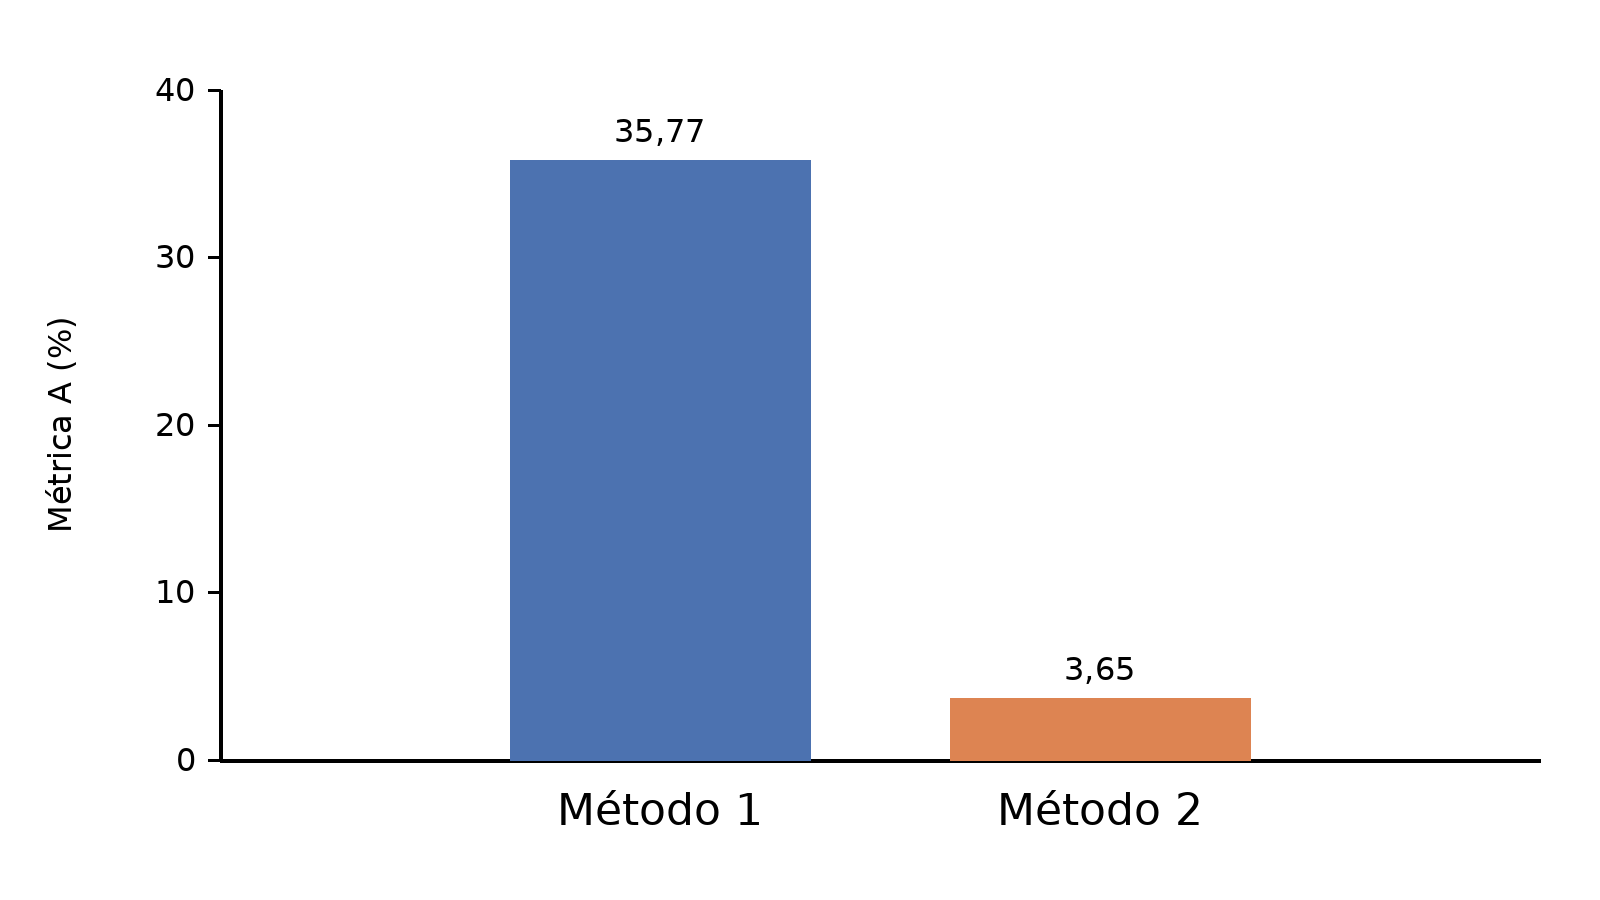
\includegraphics[width=0.9\linewidth]{figura_exemplo.png}
  \caption{Exemplo de figura com legenda descritiva, indicando
  claramente o que está sendo apresentado.}
  \label{fig:exemplo}
\end{figure}

%% ---------------------------------------------------------------
%% EXEMPLO DE TABELA
%% - Utilize o pacote "booktabs" (ja incluido) para linhas
%%   horizontais mais elegantes: \toprule, \midrule, \bottomrule.
%%   Evite linhas verticais e excesso de linhas horizontais.
%% - A legenda de tabelas (\caption) deve ficar ACIMA da tabela,
%%   ao contrario das figuras.
%% - Use \label para referenciar a tabela no texto com \ref{tab:...}.
%% ---------------------------------------------------------------
A Tabela~\ref{tab:exemplo} resume o desempenho comparativo dos
métodos avaliados.

\begin{table}[htb]
  \caption{Comparação de desempenho entre os métodos avaliados.}
  \label{tab:exemplo}
  \centering
  \begin{tabular}{lcc}
    \toprule
    \textbf{Método} & \textbf{Métrica A (\%)} & \textbf{Métrica B (s)} \\
    \midrule
    Método 1 & 35,77 & 84,2 \\
    Método 2 & 3,65  & 12,4 \\
    \bottomrule
  \end{tabular}
\end{table}


%% =====================================================================
%% 5. DISCUSSAO
%% Discuta os resultados a luz da literatura, limitacoes do estudo
%% e implicacoes praticas/teoricas.
%% =====================================================================
\section{Discussão}\label{sec:discussao}
%% ---------------------------------------------------------------
%% EXEMPLO DE CITACAO NO TEXTO
%% - Citacao entre parenteses (autor nao e o sujeito da frase):
%%     ... conforme discutido na literatura~\cite{kalman1960}.
%% - Citacao textual (autor e o sujeito da frase), referenciando
%%   diretamente pelo numero, conforme o padrao ACM/numerico:
%%     ... Kalman~\cite{kalman1960} propôs originalmente o filtro
%%     recursivo para...
%% - Multiplas referencias em uma unica citacao, separadas por
%%   virgula: \cite{kalman1960, haykin2014}
%% ---------------------------------------------------------------
Estudos anteriores mostraram resultados relevantes para o problema
abordado~\cite{kalman1960, haykin2014}. Cada referência citada no
texto DEVE constar na lista de referências ao final do artigo, e
vice-versa: toda referência listada deve ser citada pelo menos uma
vez no corpo do texto.

[Texto de discussão...]


%% =====================================================================
%% 6. CONCLUSAO E TRABALHOS FUTUROS
%% Retome os objetivos, sintetize as contribuicoes e aponte
%% direcoes futuras de pesquisa.
%% =====================================================================
\section{Conclusões e Trabalhos Futuros}\label{sec:conclusao}
[Texto de conclusão...]

\subsection{Trabalhos Futuros}\label{sec:trabalhos_futuros}
[Texto sobre trabalhos futuros...]


%% =====================================================================
%% AGRADECIMENTOS
%% ---------------------------------------------------------------------
%% NA VERSAO DE AVALIACAO (anonima): esta secao DEVE ser mantida
%% anonimizada, sem citar nomes de pessoas, financiadoras, numeros
%% de processos/bolsas ou instituicoes que possam identificar os
%% autores. Sugestao de texto padrao:
%%     "Agradecimentos omitidos para fins de avaliação cega."
%%
%% NA VERSAO FINAL: preencha normalmente os agradecimentos
%% (financiamento, bolsas, colaboradores, instituicoes de apoio etc.).
%% =====================================================================
\section*{Agradecimentos}
[Na versão de avaliação: "Agradecimentos omitidos para fins de avaliação cega."]
[Na versão final: inclua aqui os agradecimentos completos (agências de fomento, número de processo/bolsa, colaboradores, instituições de apoio etc.).]


%% =====================================================================
%% DECLARACAO DE USO DE INTELIGENCIA ARTIFICIAL
%% ---------------------------------------------------------------------
%% Secao OBRIGATORIA em ambas as versoes do artigo (avaliacao e
%% final). Os autores devem declarar, de forma clara e especifica,
%% se e como ferramentas de Inteligencia Artificial generativa
%% (ex.: ChatGPT, Copilot, Claude, Gemini, tradutores automaticos
%% com IA, entre outras) foram utilizadas na elaboracao do trabalho
%% e/ou do texto do artigo. Indique, por exemplo:
%%   - Se a ferramenta foi usada para revisao gramatical/ortografica,
%%     traducao, geracao de texto, geracao/revisao de codigo,
%%     analise de dados, geracao de figuras, etc.
%%   - Qual(is) ferramenta(s) foi(ram) utilizada(s).
%%   - Em quais etapas/secoes do trabalho a ferramenta foi empregada.
%%   - Reforce que os autores revisaram e validaram todo o conteudo
%%     gerado e assumem total responsabilidade pela integridade
%%     cientifica do trabalho.
%% Caso nenhuma ferramenta de IA generativa tenha sido utilizada,
%% declare isso explicitamente.
%% =====================================================================
\section*{Declaração de Uso de Inteligência Artificial}
[Descreva aqui, de forma objetiva, se e como ferramentas de Inteligência
Artificial generativa foram utilizadas na elaboração deste trabalho
(por exemplo: revisão textual, tradução, geração/revisão de código,
apoio à análise de dados etc.), indicando a(s) ferramenta(s)
utilizada(s) e as etapas do trabalho em que foram empregadas. Os
autores declaram ter revisado integralmente o conteúdo gerado e
assumem total responsabilidade pela precisão, originalidade e
integridade científica do trabalho. Caso nenhuma ferramenta de IA
generativa tenha sido utilizada, declare explicitamente: "Os autores
declaram que nenhuma ferramenta de Inteligência Artificial generativa
foi utilizada na elaboração deste trabalho."]


%% =====================================================================
%% REFERENCIAS
%% As referencias contam para o limite de paginas da trilha
%% escolhida (6 paginas para Artigo Completo; 3 paginas para
%% Resumo Estendido). Utilize o padrao ACM Reference Format.
%% Todas as entradas abaixo sao apenas EXEMPLOS de formatacao para
%% diferentes tipos de fonte (livro, artigo de periodico, artigo
%% em anais de evento, tese/dissertacao, pagina web); substitua
%% pelas referencias reais do seu trabalho.
%% =====================================================================
\bibliographystyle{ACM-Reference-Format}
\begin{thebibliography}{99}

%% Exemplo: livro
\bibitem{haykin2014}
S. Haykin. 2014. \textit{Adaptive Filter Theory} (5th ed.). Prentice Hall, Upper Saddle River.

%% Exemplo: artigo de periodico (journal)
\bibitem{kalman1960}
R. E. Kalman. 1960. A New Approach to Linear Filtering and Prediction Problems. \textit{Journal of Basic Engineering} 82, 1 (1960), 35--45.

%% Exemplo: artigo publicado em anais de evento/conferencia
\bibitem{exemplo_evento}
A. B. Silva, C. D. Souza. 2026. Título do Trabalho Apresentado no Evento. In \textit{Anais do XVII Computer on the Beach}. Balneário Camboriú, SC, 100--108.

%% Exemplo: tese ou dissertacao
\bibitem{exemplo_tese}
E. F. Oliveira. 2025. \textit{Título da Tese ou Dissertação}. Tese de Doutorado. Nome da Universidade.

%% Exemplo: pagina web / recurso online (incluir data de acesso quando aplicavel)
\bibitem{exemplo_web}
World Health Organization. 2019. Epilepsy: Key Facts. \url{https://www.who.int/news-room/fact-sheets/detail/epilepsy}. Acesso em: 20 ago. 2026.

\end{thebibliography}

\end{document}
